% !TEX program = XeLaTeX
% !TEX encoding = UTF-8
\documentclass[UTF8,nofonts]{ctexart}
\setCJKmainfont[BoldFont=FandolSong-Bold.otf,ItalicFont=FandolKai-Regular.otf]{FandolSong-Regular.otf}
\setCJKsansfont[BoldFont=FandolHei-Bold.otf]{FandolHei-Regular.otf}
\setCJKmonofont{FandolFang-Regular.otf}

\usepackage{url}
\usepackage{cancel}
\usepackage{xspace}
\usepackage{graphicx}
\usepackage{multicol}
\usepackage{multirow}
\usepackage{subfig}
\usepackage{amsmath}
\usepackage{amssymb}
%\usepackage[a4paper,width=180mm,top=18mm,bottom=22mm,includeheadfoot]{geometry}
\usepackage[a4paper,width=140mm,top=18mm,bottom=22mm,includeheadfoot]{geometry}
\usepackage{booktabs}
\usepackage{array}
\usepackage{verbatim}
\usepackage{caption}
%\usepackage{natbib}
\usepackage{booktabs}
\usepackage{float}
\usepackage{pdflscape}
\usepackage{mathtools}
\usepackage[usenames,dvipsnames]{xcolor}
\usepackage{afterpage}
\usepackage{pgf}
\usepackage{tikz}
\usepackage{dirtree}
\usepackage{amsfonts}
\usepackage{tkz-graph}
\usetikzlibrary{shapes.geometric}%


\title{Multilateral Token Exchange (MTX) Protocol\\一个以太坊代币的多边交易协议}
\author{ 
    dong77 <dong77@gmail.com>
    % \and
    % Haomin Li\\
    % lihaomin@zhongan.io
}

\makeatletter
\def\CTEX@section@format{\Large\bfseries}
\makeatother

\makeatletter
\newenvironment{tablehere}
  {\def\@captype{table}}
  {}

\newenvironment{figurehere}
  {\def\@captype{figure}}
  {}
\makeatother


\begin{document}
\maketitle

\begin{abstract}
本文描述一个开放的,以太坊上ERC20代币间的多边交易协议。通过该协议,可以建立去中心化且无需资产托管的交易所应用。该协议可被视为下一代数字资产交易所的开放标准之一和架构基石。传统交易所可以通过拥抱该协议改进目前交易所的撮合方式,降低用户信任成本和自身运营风险;去中心化应用(dApp)也可也以在智能合约中调用该协议的相关智能合约实现应用内的代币转换。

\end{abstract}

\section{背景介绍\label{sec:background}}

区块链作为比特币的底层技术,本质上是去中心化无信任环境中的存在性共识。存在性可应用于各种不同的数据,如股权,版权,使用权等。尽管联盟链和企业私有链中共识数据的类别正在变得越来越多样化,但这些数据的价值却有着明确的边界限制 - 只限于联盟成员间和企业内部。我们认为区块链的价值网络属性在公有链中才会的到更好的体现。根据coinmarketcap.com的统计,截止本文成稿时间,区块链上代币总市值已经超过790亿美元,以太坊区块链上承载的代币市值超过170亿美元。

区块链对各个行业都将有着深远的影响,尤其是金融领域。我们相信基于区块链的新金融会有一个明显趋势,即资产代币化(Tokenization):一方面链下资产的使用权,所有权,分红权等相关权益产通过抵押会被发行到区块链上,另一方面区块链上资产也会进行跨链发行。资产代币化的重要目标之一就是低成本,全球化,全天候的高流动性,而流动性则主要通过交易机制和交易所得以实现。

在现阶段,提供主要流动性的交易所都有非常类似的模式:交易所要求用户将法币或者代币充值到交易所的银行或区块链账户中,然后交易所在自己中心服务器的虚拟账户系统中为用户进行IOU记账。用户实际交易的是这些IOU。为了将IOU兑换成法币或区块链代币,用户需要向交易所提出提现请求,提现成功后,才算真正交易完成。在这个过程中,交易所替用户安全保管资产的能力是用户最大的风险;同时用户还需担心交易所运营者的商业道德问题,比如挪用资金造成资不抵债等。2014年2月当时世界最大规模的比特币交易所运营商Mt.Gox的85万个比特币被盗一空,公司向日本东京地方法院申请破产保护。该公司的用户至今仍在等待其返还尚未被盗的少量比特币。随着调查的不断进行Mt.Gox被曝出所谓的比特币被盗其实是监守自盗。85万个“被偷窃”的比特币中,实际上因外部盗窃失踪的仅为7000个。而包括比特币存钱罐和ShapeShift在内的平台被盗事件也被曝出涉及内部人士。2016年8月最大的美元比特币交易平台香港的Bitfinex由于网站出现安全漏洞,导致用户持有的比特币被盗,被盗的比特币共119756枚,总价值约为6500万美元。随后该公司决定由所有用户共同分担损失以避免其破产。交易所缺失的资产保管能力和监守自盗的败坏的商业道德,一方面反映出比特币在各个国家监管政策的缺失与漏洞,另一方面也证实中心化交易所模式的固有风险。

基于区块链的去中心化交易机制就是为了彻底解决上述问题。去中心化交易的核心优势之一是避免任何资产被托管,因此资产就不存在被盗的可能性,这会极大降低用户对交易所的信任成本;这种交易机制的另一个优势是没有地缘和时间限制,以及极高的透明性和可追溯性。这些特点会促使交易整体具有更大的流动性和更小的买卖价差。

\section{相关工作\label{sec:existingworks}}
%[几个段落:介绍早期区块链上交易所的尝试,特别是Ripple的机制。]

此前,社区已经有过一些基于区块链搭建去中心化的交易所的尝试,如ripple、比特股、闪电网络等。这些项目通过不同的方法实现虚拟资产交易,优化性能。

Ripple \cite{schwartz2014ripple} 是一个去中心化的银行系统间清算协议,为方便的在全世界范围转账支付而设计的,具有快速、方便、超低费用的优点。Ripple提出了一项Interledger \cite{thomas2015protocol} 协议(ILP)实现跨账本的资产交易,无论是分布式的,还是传统的中心化账本。ILP 本身并不是一个账本,相反,它提供了一个顶层加密托管系统,在称之为“连接者”的中介机构的帮助下,可以让资金在各账本之间进行流动。

比特股 \cite{schuh2015bitshares}\cite{schuhbitshares}  是一个基于区块链的开发平台,任何个人和机构都可以在此平台上自由地进行转账、借贷、发行资产等,也可以基于这个平台快速搭建出去中心化的金融服务平台等。BitShares 内置的去中心化交易所(DEX),让数字资产的交易撮合和交割完全发生在链上,并通过内置智能合约锚定其他资产,如法币、比特币、黄金、白银等。

闪电网络(Lightning Network)\cite{poon2015bitcoin}是一个去中心化的系统。闪电网络的卓越之处在于,无需信任对方以及第三方即可实现实时的、海量的交易网络。闪电网络提供了一个可扩展的微支付通道网络。交易双方若在区块链上预先设有支付通道,就可以多次、高频、双向地通过轧差方式实现瞬间确认的微支付;双方若无直接的点对点支付通道,只要网络中存在一条连通双方的、由多个支付通道构成的支付路径,闪电网络也可以利用这条支付路径实现资金在双方之间的可靠转移。

%Openledger是一个新型去中心化交易平台。它允许用户将比特币兑换成法币锚定的 SmartCoins,SmartCoins 可以直接通过 paypal、 瑞波网关以及 CCEDK 的 NanoCard 兑换成现金。需要注意的是,Openledger在很大程度上依赖于比特股 2.0平台以及 Cryptonomex 开发的 Graphene Toolkit。因此,Openledger平台的性能取决于Graphene Toolkit的性能和比特股 2.0平台的性能。

%[几个段落:介绍一些automatic market maker算法,包括Bancor协议,{Price Evolution in a Continuous Double Auction Prediction Market With a Scoring-Rule Based Market Maker}, {Hanson, R. 2003a. Book orders for market scoring rules. George Manson University.}]

在经济学中的资产交易方面有一个经典问题叫做“双重需求巧合”,Bancor协议引入了一种技术解决方案,通过使用以区块链为基础的智能合约和储备货币来解决这个问题。任何人都可以通过这个协议创建代币,代币以预先设置的比率来持有一种或几种其它代币作为自己的储备金。这些储备代币可以是法币、数字化资产或其它加密货币。通过使用这些储备金,不论有没有交易,新创建的代币都可以获得价值。此外,不论有没有买家,这些新创建的代币都可以随时兑换回其储备代币。

%[一个稍长的段落:介绍0x协议,指明其缺点,比如:1)taker负责匹配订单,要求taker在线,撮合实时性差因此撮合价格无法及时优化,2)实际就是简单的OTC方式,没法实现复杂订单的撮合,3)交易所之间没有明确的竞争激励机制,4)没有考虑旷工的利益。]

0x \cite{warren20170x} 是一个可以在以太坊区块链上进行 ERC20 代币对等交易的开放式协议。该协议旨在成为通用开放标准,作为可与其他协议组合的基本模块,用以驱动越来越复杂的区块链应用程序。由于它使用的是公开访问的智能合约系统,因此可以作为各种 dApps 的共享基础架构。而从长远来看,开放式技术标准相比封闭模式具有更大的优势,随着每个月有更多的资产在区块链上被代币化,也有更多的 dApps 需要使用这些不同的代币,开放式标准也因此变得更加重要。此外,由 dApps 耦合到其底层协议所导致的智能合约冗余也是未来区块链协议开发的主要障碍,因此在标准化之余,我们还需要一个合适的解耦方式。0x 协议试图将信息交换功能从应用层拉到协议层,推动 dApps 之间的互操作性。然而,0x协议具有以下局限性:taker必须在线匹配订单,这导致撮合实时性差,难以优化成交价格;0x协议采用的是简单的OTC方式,无法法实现复杂订单的撮合;不同交易所之间没有明确的竞争激励机制;没有考虑了矿工的利益。
%[几个段落:介绍早期区块链上交易所的尝试,特别是Ripple的机制。
%
%
%[几个段落:介绍一些automatic market maker算法,包括Bancor协议,{Price Evolution in a Continuous Double Auction Prediction Market With a Scoring-Rule Based Market Maker}, {Hanson, R. 2003a. Book orders for market scoring rules. George Manson University.}]
%
%[一个稍长的段落:介绍0x协议,指明其缺点,比如:1)taker负责匹配订单,要求taker在线,撮合实时性差因此撮合价格无法及时优化,2)实际就是简单的OTC方式,没法实现复杂订单的撮合,3)交易所之间没有明确的竞争激励机制,4)没有考虑旷工的利益。]

我们受0x协议和闪电网络的启发,提出一个以太坊上ERC20代币间交易协议。通过该协议,代币持有者可以通过数字签名授权指定的一个或多个交易所帮助自己撮合订单,并将该订单在链下广播给交易所;交易所会使用与MTX智能合约中相同的逻辑对多个订单进行匹配,通过数字签名生成区块链交易,并负责将交易广播到以太坊网络,并通过触发智能合约实时完成代币在相关交易方间的清算和转账。

\section{MTX协议\label{sec:protocol}}

\begin{center}
\begin{figurehere}
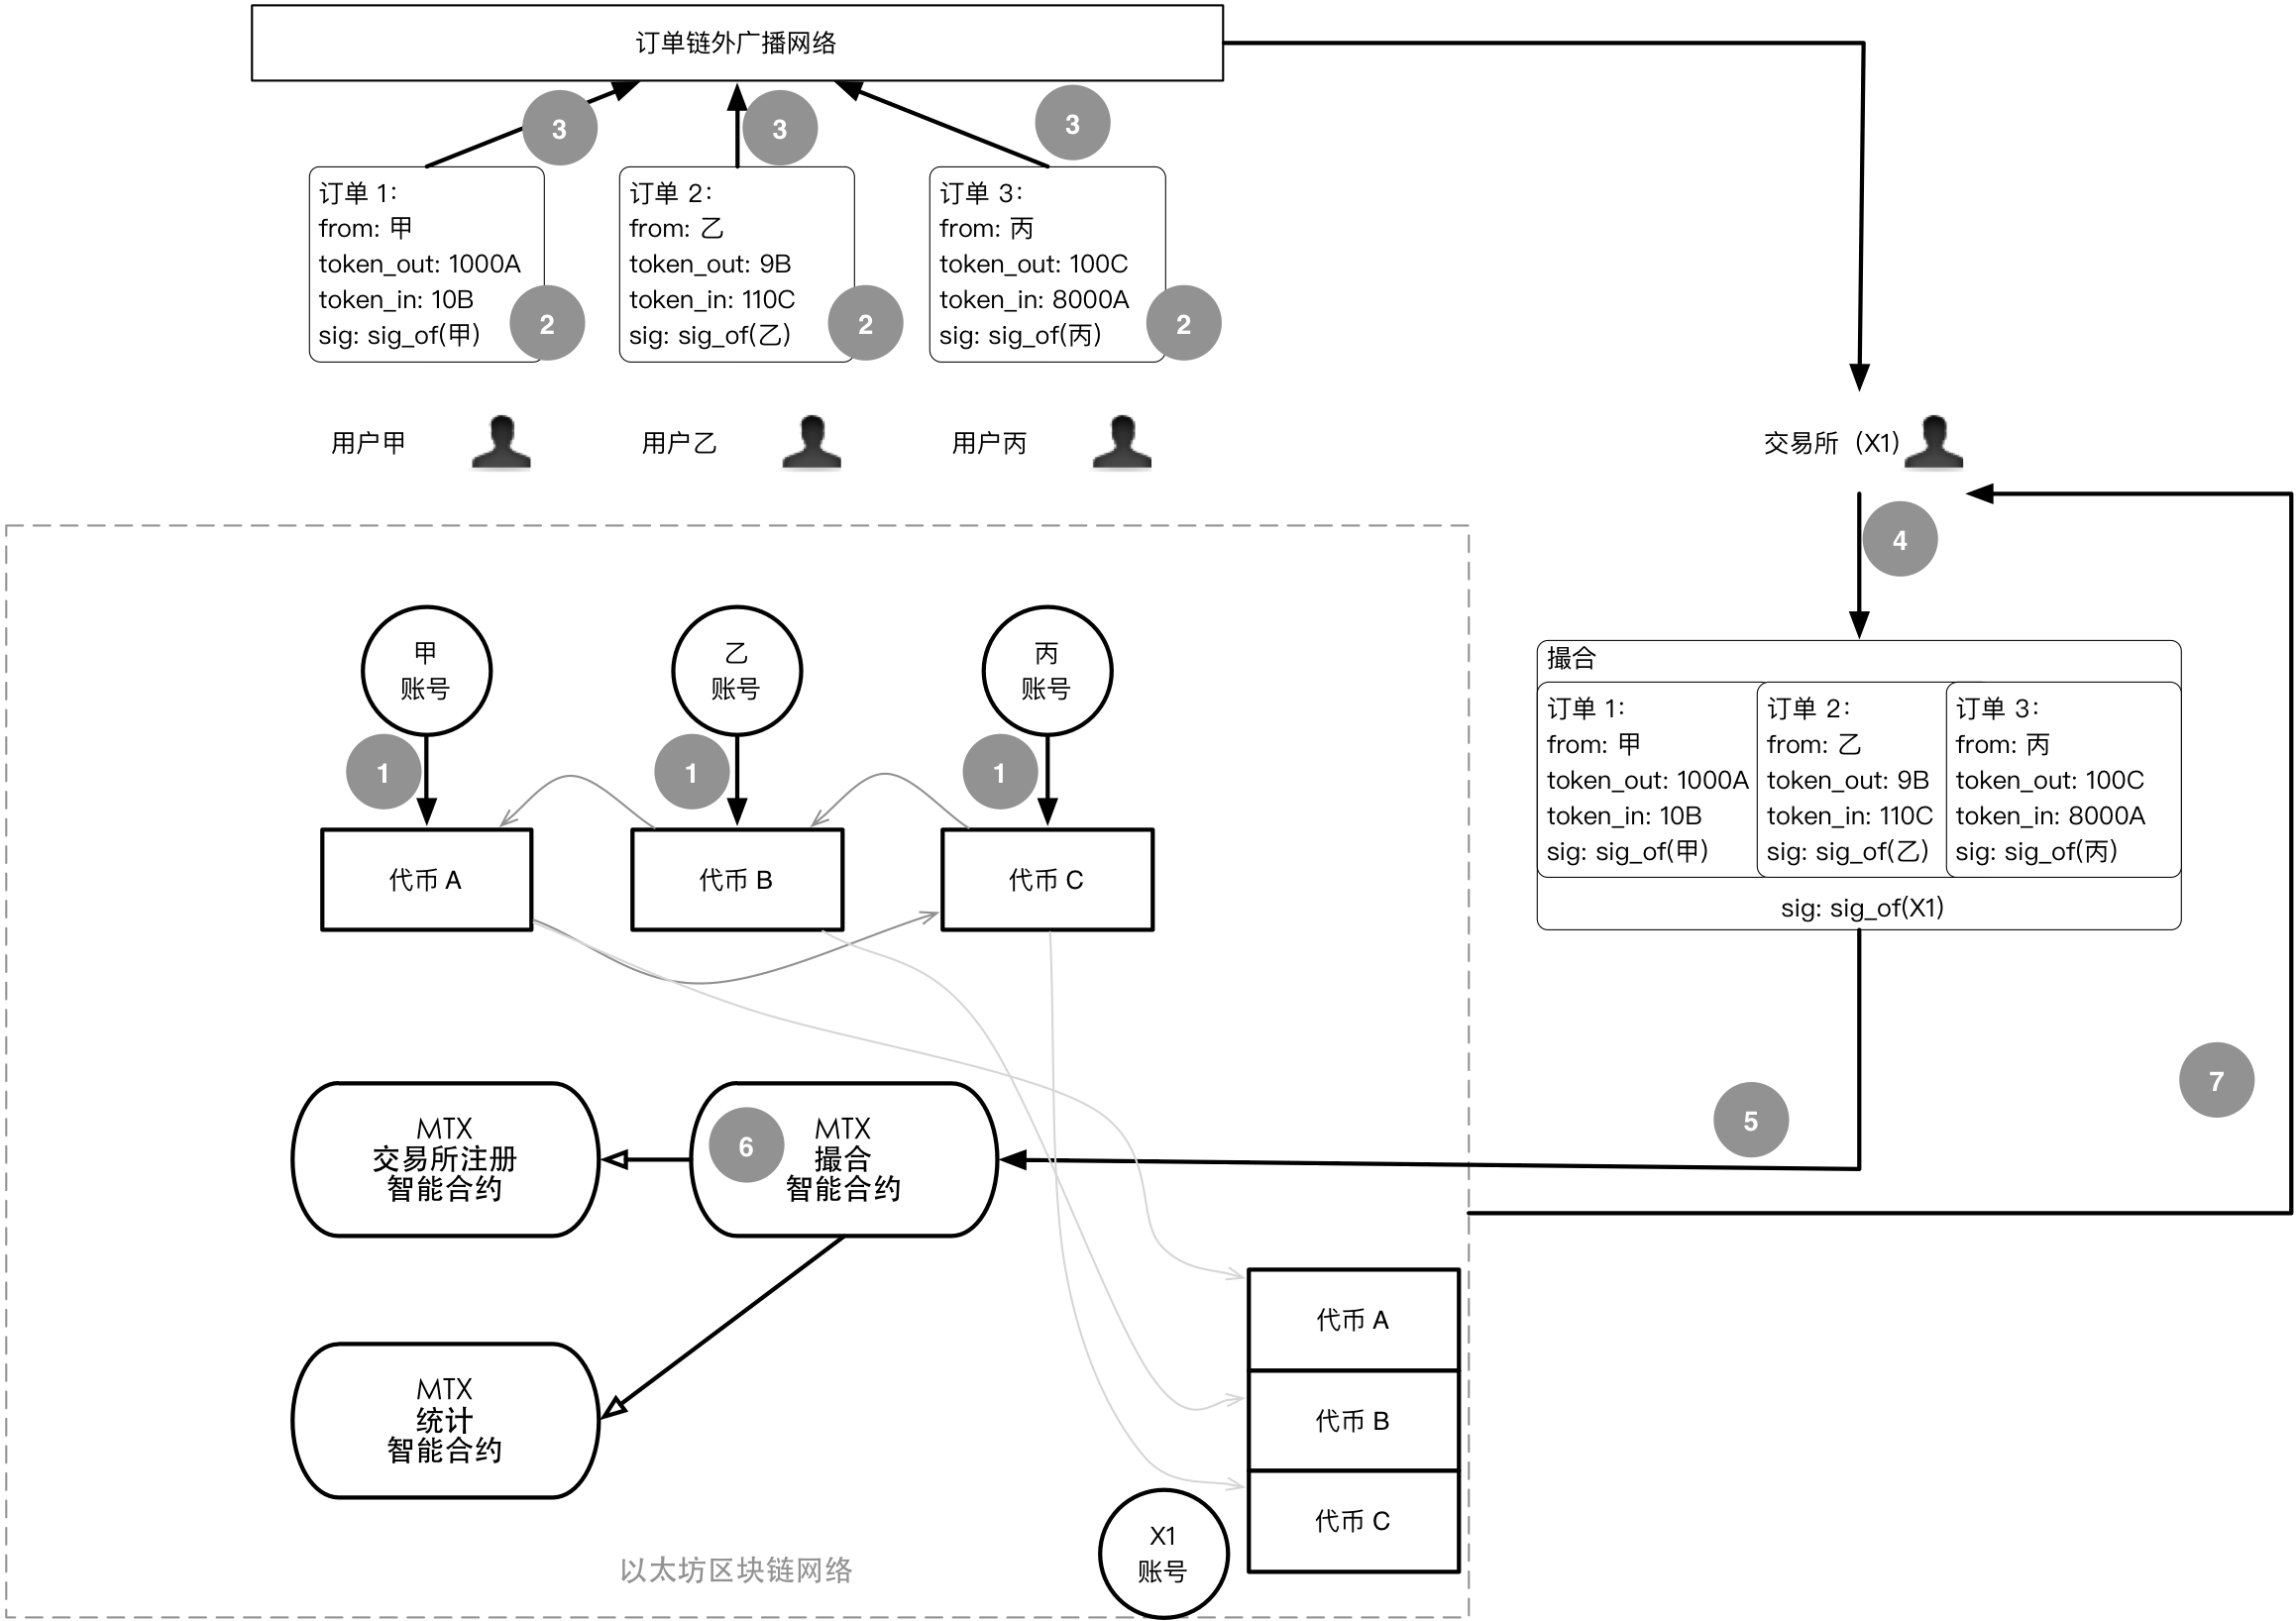
\includegraphics[height=10cm]{images/mtx-protocol.png}
\caption{MTX协议:图中示例一个三边交易的撮合}
\label{fig:mtxprotocol}
\end{figurehere}
\end{center}

采用MTX协议的撮合交易过程如下:

\begin{enumerate}
	\item 用户甲,乙,丙分别对MTX撮合智能合约(Matchengine Contract)授权,授权后该合约可对用户指定代币账号做不超过一定额度的转出操作。在上面实例中,合约可最多从用户甲的账号转出1000个A,从用户乙账户转出9个B,从用户丙账户转出100个C;
	\item 用户甲,乙,丙分别生成自己的订单,并用私钥对其进行数字签名。订单的表示不再区分买单和卖单,所有订单都可以视为是“交换单”: 甲的订单声明:甲愿意支出不多于1000个A,得到尽可能多但不少于10个B;如果是部分成交,那么A到B的兑换率不得低于1000/10,即100.0。订单中还可以包含很多其它的参数,我们在\ref{sec:dataformat}中会进一步说明;
	\item 甲,乙,丙分别将自己的订单通过适当的方式广播或定向发送给交易所;
	\item 交易所X1收到上述三个订单,将订单放到三个OrderBook中,并实时通过区块链数据更新订单状态。同时交易所不断计算寻找能够撮合的订单组。一旦确定三个订单的当前状态可以撮合成功,且收益(交易手续费,分润,并去除预估的以太坊gas费)满足预期,则将三个订单组装成一个撮合交易(Match Transaction);
	\item 交易所对撮合交易签名后发送到MTX的撮合智能合约;
	\item 撮合智能合约验证四方签名,之后验证三个订单(的最新状态)是否可以真正成交。若无法成交,合约终止;否则智能合约分别计算出甲乙丙三方各自需要支出的金额,以及交易所X1该收取的费用,并且实时将甲乙丙账号中的资产进行互转,同时支付费用给交易所X1完成清算。在交易过程中,撮合智能合约还会调用MTX注册智能合约(Exchange Registration Contract)来检查交易所是否有权进行撮合,以及费用声明;在交易完成前,还会调用MTX统计智能合约(Trade Stats Contract)对交易所撮合统计做更新,同时更新不同代币间兑换率的变化情况。
	\item 交易所监听新的区块,并根据其中的数据更新相关订单的状态,并根据全部的Order Book进行新一轮撮合服务。
\end{enumerate}

在传统交易所模型中,被撮合的两方中先下单的为Maker,后下单的为Taker。因为Maker创造流动性而Taker销毁流动性,因此多数交易所的成交价时候会给Maker折扣价,甚至直接采用Maker的价格作为成交价格。与之相比,MTX采用的是All-Maker模型,这是由于在去中心化环境中,很难严格界定哪个单是真正意义上最早的单,因此把所有订单都是被视为Maker既可以简化判断,又可以在计算成交价的时候不偏向任何一方,使得交易更加公平。

MTX协议的另一个显著特点是消除了“交易对(Trading Pair)”的概念。一个从A到B的订单不一定要一个从B到A反向的订单才能撮合,只要有一个交换环路被发现,就可以撮合成功。也可以说传统交易所的市场概念是多边交易闭环的一个最简单的特例。我们后续用订单中两个代币类型的组合来表示订单的类型。

\subsection{定价机制\label{sec:pricediscovery}}

%[段落:讲讲中心和交易所的定价模型,以及为什么不适合于去中心化交易所 double action vs taker maker]
%
%[段落,讲讲我们的定价模型:我们属于double auction模型,采用中间级成交,同时讲讲交易所收费]
%
%[段落:价格发现机制的理论证明]
%
%[段落:成绩额度的计算]
%
%[段落:交易所费用的计算]
在整个生态中,负责撮合的交易所处于核心地位,为了鼓励交易所更高效的完成撮合,我们设计了一套针对交易所的经济激励机制。交易所的收入来自两部分:一部分是来自交易单的手续费,每一个交易单都需要支付一定代币作为手续费,手续费是奖励给交易所的,以激励交易所撮合更多的交易;另一部分是撮合交易的利差提成,当交易所撮合交易产生利差时,交易所可以按比例从中获得提成,以激励交易所撮合利差更高的交易。

交易所上传一个交易闭环$T_0 \rightarrow T_1 \rightarrow ... \rightarrow T_{n-1} \rightarrow T_{0}$并撮合成功,假设每一单$T_{i}$$(i\in{0,...,n-1})$对应的手续费是$fee_{i}$,那么交易所的手续费收入则为
$
\sum^{n-1}_{i=0}fee_{i}\text{。}
$
交易所的另一部分收入来自于撮合交易的利润提成。如果按照原价每一单$T_{i}$$(i\in{0,...,n-1})$够成交$Amt_{i}$,而按撮合后的折价能够成交$Amt'_{i}$,那么交易所就可以从每一单的利润中获得$(Amt'_{i}-Amt_{i})*x\%$的提成,其中$x\%$是提成的比例,因此交易所的撮合交易提成是
$
\sum^{n-1}_{i=0}(Amt'_{i}-Amt_{i})*x\%\text{。}
$
因此交易所的总利润为
$$
\text{总利润} = \sum^{n-1}_{i=0}fee_{i}+(Amt'_{i}-Amt_{i})*x\%\text{。}
$$
交易所在撮合时会综合考虑这两方面的收入做出撮合交易的决策,以优化利润总额。

(王辉:这个地方$(Amt)$概念有点模糊,能否用实际成交额 T,订单卖出代币余额O, 订单兑换率R,和实际兑换率R'来计算,这样分成就是就是 Max(O - T*R', T(R-R')*feePercentage) )

\subsection{交易环路\label{sec:tradecircle}}

协议要求一个合法的交易环路必须具有下列属性:

\begin{itemize}
	\item 它的订单子集无法组成更小的可交易环路;
	\item 它上面订单的兑换率之积不大于1;
\end{itemize}

\subsection{市场深度计算\label{sec:pricediscovery}}

\subsection{数据格式\label{sec:dataformat}}

由于采用All-Maker模型,所有订单都可以用同一个结构表示。该结构包含订单本身的各种参数数据和数字签名。在签名前,现将订单参数数据连接成一个字节数组,通过Keccak SHA3方法对这个字节数组做散列计算得到订单的哈希,之后用账户私钥对这个哈希进行ECDSA签名。


\begin{verbatim}
message Order {
  address protocol;   // MTX协议入口智能合约地址
  address owner;      // 该订单所有者(发起者)地址
  address outToken;   // 卖出ERC20代币智能合约地址
  address inToken;    // 买入ERC20代币智能合约地址
  uint256 outAmount;  // 卖出ERC20代币数量
  uint256 inAmount;   // 买入ERC20代币数量
  unit256 expiration  // 过期时间
  unit256 fee;        // 交易总费用(MTX Token),部分成交的费用按该次匹
                      // 配实际卖出货币额与outAmount比例计算。
  uint8 savingSharePercentage; // fee余额不足时支付给交易所的分润比例
  bytes signature;    // 上面数据的ECDSA签名,也可以用作订单ID
}	
\end{verbatim}

订单中虽然没有明确指定价格,但我们可以通过计算\verb|outAmount/inAmount|来得到一个订单兑换率\verb|R|。该兑换率隐含地要求所有实际撮合成交的兑换率不得大于\verb|R|。一个好的交易所UI应该允许用户指定\verb|outAmount|,\verb|inAmount|,和传统意义的买入价或卖出价这三个数据的任意两个来计算缺失的\verb|outAmount|或\verb|outAmount|值。

订单实际上可以有两种不同的“完全成交”定义:一种定义是只有卖出代币达到了\verb|outAmount|才算完全成交;另一种定义在之前的基础上允许买入代币累计金额达到\verb|inAmount|也算完全成交。我们可以在订单中引入一个参数告诉交易所和撮合智能合约选择哪种完全成交定义。在第一版本的实现中,我们先支持第一种定义。

\begin{verbatim}
message Match {
    Order[] orders;     // 该次匹配的所有订单
    address feeRecipient; // 费用收取地址
    bytes signature;      // 上面数据的ECDSA签名
}
\end{verbatim}

一次撮合中包含的订单应该形成一个可交易环路,并且该环路上同一类型的订单只能有一个 --- 理论上可以将这个限制去掉,不过这会让撮合智能合约更加复杂,因此初期不予支持。放开这个限制的好处是一次撮合中将将更多订单完全成交。


[段落:讲讲订单状态]

[段落:部分成交和取消订单]

[段落:讲讲撮合成功条件]


[段落:代币名字注册合约]

[段落:交易所注册合约]

[段落:交易所统计合约]

[段落:token兑换率统计合约]


\subsection{交易所\label{sec:exchange}}

交易所为用户提供的核心价值是价格发现和交易撮合。交易所的价格发现服务通过汇聚尽可能多的订单,并且对订单进行状态追踪和更新,按照兑换率排序形成多个全局的多Orderbook,同时根据多个Orderbook,计算出任何两个代币之间的兑换率历史和特定的统计指标,比如最新兑换率,滑动成交趋势等等。交易撮合服务建立在价格发现服务的基础之上,通过优化多边交易环路发现算法,尽可能快地将撮合提交到以太坊区块链,通过智能合约做撮合验证和清算。我们预测交易所的第三个重要服务是代币发行和承兑服务,将以太坊链外资产引入到以太坊网络。不过这个服务和本文的协议相关性不大,我们不做进一步阐释。

交易所撮合服务的收入是撮合手续费或分润。订单中可以指定一个\verb|fee|,这是该订单在完全成交后愿意支付给交易所的费用 --- 以协议代币计价。如果订单是部分成交,则按照相应比例支付\verb|fee|的一部分给交易所。如果该订单拥有者账户中用于支付该次撮合的协议代币不足,撮合智能合约会通过分润的计算来支付订单中的一部分卖出货币给交易所。

交易所并不能保证每一个撮合都是盈利的。一方面的原因可能是成本过高,因为交易所为了激励旷工有限打包自己的撮合交易到区块链,因此可能根据预期的收益调高gas,这部分gas是用以太计费的,而以太和撮合中代币的价格相对价格有可能有交大浮动,从而造成gas实际成本更好。另一方面的原因是收入没有达到预期,比如交易所把撮合广播到区块链后,该撮合的某个订单的卖出货币被部分或者全部转移到另一个地址,从而造成整个撮合交易不被智能合约接受。类似这样的原因还有很多,因此交易所的每次撮合广播都是根据自己的经验和算法,最大化长期利益的概率游戏。不过也不用担心,实际上交易所和订单发起者是双向选择的关系:交易所只会选择有利可图的订单;而订单发起者只会选择撮合速度最快,撮合价格最理想的交易所 --- 这是通过MTX的统计合约数据得到支撑的。

[段落:价值,收入,相互竞争,交易所时间和利润的平衡,旷工对撮合的选择和利益]

[段落:交易所评分]

[段落:交易所如何实现短期利润最大化]

[段落:交易所的信用积累]

[段落:交易所的初创成本]


[段落:如何激励转发订单???]

\section{协议代币\label{sec:exchangetoken}}

[段落:代币用于支付交易费,更节约成本]

[段落:交易所购买代币进行注册的抵押]

[段落:协议代币也是ERC20,可以同样方式交易,因此生态是个完整闭环]

\section{鸣谢\label{sec:acknowledgement}}

\bibliography{whitepaper}
\bibliographystyle{acm}

\end{document} 